\documentclass[10pt,journal,compsoc,onecolumn]{IEEEtran}
\usepackage[utf8]{inputenc}
\usepackage{amsmath,amsfonts,amssymb}
\usepackage{amsthm}
\usepackage{graphicx}
\usepackage{cite}
\usepackage{textcomp}
\usepackage{tikz}
\usetikzlibrary{arrows,positioning,shapes.geometric}
\usepackage{booktabs}
\usepackage{url}

\newtheorem{theorem}{Theorem}
\newtheorem{lemma}[theorem]{Lemma}
\newtheorem{definition}[theorem]{Definition}
\newtheorem{corollary}[theorem]{Corollary}

\begin{document}

\title{A Formal Algorithmic Analysis of Stack Data Structures: Implementations, Applications, and Monotonic Stack Techniques}

\IEEEtitleabstractindextext{%
\begin{abstract}
Stacks represent a fundamental abstract data type operating under the Last-In, First-Out (LIFO) protocol. This paper presents a formal analysis and reference implementations of stack structures, analyzing their memory allocation schemes across stack and heap boundaries. We cover the core push, pop, peek, and status queries under strict constant-time O(1) bounds. We then formalize two primary applications: parenthesis matching and postfix expression evaluation, detailing their state space and transition mechanics. Finally, we investigate the Monotonic Stack paradigm for solving the Nearest Smaller Element (NSE) problem. We prove that while the naive brute-force method incurs $O(N^2)$ time, the monotonic stack algorithm achieves optimal $O(N)$ time complexity and $O(N)$ space complexity. Java reference implementations and formal correctness arguments are provided.
\end{abstract}

\begin{IEEEkeywords}
linked list, deep copy, random pointer, hash map, node interleaving, Java, algorithm analysis, computational complexity
\end{IEEEkeywords}
}

\maketitle
\IEEEdisplaynontitleabstractindextext
\IEEEpeerreviewmaketitle

\section{Introduction}
Stacks are a fundamental linear data structure in computer science, operating under the Last-In, First-Out (LIFO) access discipline. In a LIFO structure, the element last added to the stack is the first one to be removed. This simple yet powerful mechanism underpins key computer systems operations, from expression parsing and recursive function invocation to memory call stacks and transaction undo/redo history.

This paper provides a rigorous algorithmic treatment of the stack data structure. We define its abstract data type (ADT) and evaluate the performance of array-based and linked list-based implementations. We formalize two core stack applications: parenthesis matching and postfix expression evaluation, detailing their state transition mechanisms. Finally, we explore the Monotonic Stack paradigm, presenting an optimal $O(N)$ solver for the Nearest Smaller Element (NSE) problem, contrasted against the naive $O(N^2)$ brute-force solution.

\section{Stack Abstract Data Type (ADT)}
A stack $S$ is a dynamic set of elements supporting a restricted set of access operations. Formally, we define the stack state as a sequence of elements $\langle s_1, s_2, \ldots, s_t \rangle$, where $s_t$ represents the top of the stack and $s_1$ represents the bottom. The integer $t \ge 0$ represents the stack pointer (current size).

The stack ADT supports the following operators:
\begin{itemize}
    \item $\mathrm{Push}(S, x)$: Inserts element $x$ onto the top of the stack.
    $\langle s_1, \ldots, s_t \rangle \xrightarrow{\mathrm{push}(x)} \langle s_1, \ldots, s_t, x \rangle$.
    \item $\mathrm{Pop}(S)$: Removes and returns the top element $s_t$.
    $\langle s_1, \ldots, s_t \rangle \xrightarrow{\mathrm{pop}()} \langle s_1, \ldots, s_{t-1} \rangle$.
    \item $\mathrm{Peek}(S)$: Returns the top element $s_t$ without modifying the stack.
    \item $\mathrm{IsEmpty}(S)$: Returns true if $t = 0$, else false.
\end{itemize}

\begin{figure}[htbp]
\centering
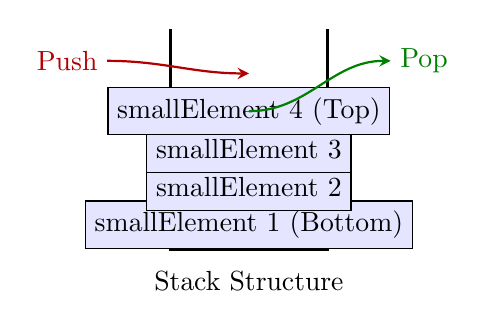
\begin{tikzpicture}[
  stacknode/.style={draw, rectangle, minimum width=2.5cm, minimum height=0.6cm, fill=blue!10, font=small},
  scale=0.8
]
% Draw stack bucket
\draw[very thick] (0, 3.5) -- (0, 0) -- (2.5, 0) -- (2.5, 3.5);

% Draw elements
\node[stacknode] at (1.25, 0.4) {Element 1 (Bottom)};
\node[stacknode] at (1.25, 1.0) {Element 2};
\node[stacknode] at (1.25, 1.6) {Element 3};
\node[stacknode] at (1.25, 2.2) {Element 4 (Top)};

% Push/Pop arrows
\draw[->, >=stealth, thick, red!70!black] (-1, 3.0) to [out=0, in=180] (1.25, 2.8);
\node[left, red!70!black] at (-1, 3.0) {Push};

\draw[->, >=stealth, thick, green!50!black] (1.25, 2.2) to [out=0, in=180] (3.5, 3.0);
\node[right, green!50!black] at (3.5, 3.0) {Pop};

\node at (1.25, -0.5) {Stack Structure};
\end{tikzpicture}
\caption{Visual representation of a Stack operating under the LIFO principle.}
\label{fig:stack}
\end{figure}

\subsection{Implementation Paradigms}
Stacks are typically implemented using two primary physical data structures:
\begin{enumerate}
    \item \textbf{Sequential Array Representation:} Elements are stored in contiguous memory. A cursor variable $t$ tracks the top index.
    \item \textbf{Linked List Representation:} Elements are stored in dynamic heap-allocated nodes, where each node points to its predecessor.
\end{enumerate}

\subsubsection{Array-based Implementation}
In an array-based stack of fixed capacity $C$, pushing to a full stack ($t = C-1$) triggers a \textit{Stack Overflow} exception. Conversely, popping from an empty stack ($t = -1$) triggers a \textit{Stack Underflow} exception. To achieve dynamic scaling, one can double the array capacity when the stack is full, yielding an amortized time complexity of $O(1)$ for push operations.

\subsubsection{Linked List-based Implementation}
A linked list-based stack resolves the fixed capacity constraint. Every push allocates a new node on the heap and adjusts pointers:
\begin{verbatim}
void push(Node** top, int data) {
    Node* newNode = (Node*)malloc(sizeof(Node));
    if (newNode == NULL) return; // Out of memory
    newNode->data = data;
    newNode->next = *top;
    *top = newNode;
}
\end{verbatim}
This implementation guarantees $O(1)$ worst-case time for all operations but incurs an $O(N)$ pointer storage overhead.

\subsection{Asymptotic Complexity Analysis}
Table~\ref{tab:complexities} summarizes the asymptotic time and space bounds for both implementations.

\begin{table}[htbp]
\centering
\caption{Asymptotic Bounds of Stack Operations.}
\label{tab:complexities}
\begin{tabular}{lllll}
\toprule
Operation & \multicolumn{2}{c}{Array-based (Resizing)} & \multicolumn{2}{c}{Linked List-based} \\
\cmidrule(lr){2-3}\cmidrule(lr){4-5}
& Time & Space & Time & Space \\
\midrule
Push & $O(1)$ amortized & $O(1)$ auxiliary & $O(1)$ worst-case & $O(1)$ auxiliary \\
Pop & $O(1)$ worst-case & $O(1)$ auxiliary & $O(1)$ worst-case & $O(1)$ auxiliary \\
Peek & $O(1)$ worst-case & $O(1)$ auxiliary & $O(1)$ worst-case & $O(1)$ auxiliary \\
IsEmpty & $O(1)$ worst-case & $O(1)$ auxiliary & $O(1)$ worst-case & $O(1)$ auxiliary \\
\bottomrule
\end{tabular}
\end{table}

\section{Application I: Balanced Parenthesis Matching}
A common application of stacks is verifying if a sequence of parentheses is balanced. Let $\Sigma = \{\text{(}, \text{)}, \text{\{}, \text{\}}, \text{[}, \text{]}\}\}$ be the alphabet. Let $S \in \Sigma^*$ be a string of length $N$. Let $LOB = \{\text{(}, \text{\{}, \text{[}\}\}$ be the set of left (opening) brackets and $ROB = \{\text{)}, \text{\}}, \text{]}\}\}$ be the corresponding right (closing) brackets.

\subsection{Algorithm and State Transitions}
The stack-based balanced parenthesis solver parses the input string $S$ from left to right.
\begin{enumerate}
    \item If $S[i] \in LOB$, push $S[i]$ onto the stack.
    \item If $S[i] \in ROB$, peek the stack. If the stack is empty, or the top element does not match the type of $S[i]$ (e.g., $S[i] = \text{)}$ but top is $\text{[}$), the sequence is unbalanced (returns false). Otherwise, pop the stack.
    \item After processing all characters, the sequence is balanced if and only if the stack is empty.
\end{enumerate}

The rule "last opened bracket must be closed first" is mathematically maintained because the stack acts as a LIFO queue.

\subsection{Java Implementation}
The Java implementation of the parenthesis checker is as follows:
\begin{verbatim}
import java.util.Stack;

public class ParenthesisMatcher {
    public static boolean isValid(String seq) {
        Stack<Character> st = new Stack<>();
        for (int i = 0; i < seq.length(); i++) {
            char ch = seq.charAt(i);
            if (ch == '(' || ch == '{' || ch == '[') {
                st.push(ch);
            } else {
                if (st.isEmpty()) return false;
                char top = st.peek();
                if ((ch == ')' && top == '(') ||
                    (ch == '}' && top == '{') ||
                    (ch == ']' && top == '[')) {
                    st.pop();
                } else {
                    return false;
                }
            }
        }
        return st.isEmpty();
    }
}
\end{verbatim}

\subsection{Complexity Analysis}
The time complexity is $O(N)$ as we make a single linear pass over the input string. The auxiliary space complexity is $O(N)$ in the worst case where all elements in the input string are opening brackets (e.g., $S = \text{(((((}$), resulting in all characters being pushed onto the stack.

\section{Application II: Postfix Expression Evaluation}
Arithmetic expressions are traditionally written in infix notation (e.g., $A + B$), where operators sit between operands. Postfix notation (e.g., $A\ B\ +$), also known as Reverse Polish Notation (RPN), places operators after their operands. This representation eliminates the need for parenthetical grouping and operator precedence hierarchies.

\subsection{The Postfix Evaluation Algorithm}
A stack is used to evaluate a postfix expression $E$:
\begin{enumerate}
    \item Scan the postfix expression from left to right.
    \item If the token is an operand, push it onto the stack.
    \item If the token is a binary operator $\odot$:
        \begin{enumerate}
            \item Pop the top element $op_2$ (second operand).
            \item Pop the next top element $op_1$ (first operand).
            \item Perform the operation $res = op_1 \odot op_2$.
            \item Push $res$ back onto the stack.
        \end{enumerate}
    \item After scanning the entire expression, the final result is popped from the stack.
\end{enumerate}

\subsection{Illustrative Execution Trace}
We trace the evaluation of the expression $E = \langle 3, 5, +, 2, -, 2, 5, *, - \rangle$ in Table~\ref{tab:trace}.

\begin{table}[htbp]
\centering
\caption{Dry-run evaluation of postfix expression $3\ 5\ +\ 2\ -\ 2\ 5\ *\ -$.}
\label{tab:trace}
\begin{tabular}{cllll}
\toprule
Step & Token & Action & Operands Popped & Stack State (bottom to top) \\
\midrule
0 & - & Initialize & - & $\langle \rangle$ \\
1 & 3 & Push Operand & - & $\langle 3 \rangle$ \\
2 & 5 & Push Operand & - & $\langle 3, 5 \rangle$ \\
3 & + & Add & $op_2=5, op_1=3$ & $\langle 8 \rangle$ \\
4 & 2 & Push Operand & - & $\langle 8, 2 \rangle$ \\
5 & - & Subtract & $op_2=2, op_1=8$ & $\langle 6 \rangle$ \\
6 & 2 & Push Operand & - & $\langle 6, 2 \rangle$ \\
7 & 5 & Push Operand & - & $\langle 6, 2, 5 \rangle$ \\
8 & * & Multiply & $op_2=5, op_1=2$ & $\langle 6, 10 \rangle$ \\
9 & - & Subtract & $op_2=10, op_1=6$ & $\langle -4 \rangle$ \\
\bottomrule
\end{tabular}
\end{table}

The final value at step 9 is $-4$.

\subsection{Java Implementation}
The Java reference implementation is:
\begin{verbatim}
import java.util.Stack;

public class PostfixEvaluator {
    public static int evaluate(String[] tokens) {
        Stack<Integer> st = new Stack<>();
        for (String t : tokens) {
            if (t.equals("+") || t.equals("-") || 
                t.equals("*") || t.equals("/")) {
                int op2 = st.pop();
                int op1 = st.pop();
                if (t.equals("+")) st.push(op1 + op2);
                else if (t.equals("-")) st.push(op1 - op2);
                else if (t.equals("*")) st.push(op1 * op2);
                else if (t.equals("/")) st.push(op1 / op2);
            } else {
                st.push(Integer.parseInt(t));
            }
        }
        return st.pop();
    }
}
\end{verbatim}

\subsection{Complexity Analysis}
The time complexity is $O(N)$ since each token is processed exactly once. The space complexity is $O(N)$ auxiliary to store the operands on the stack.

\section{Monotonic Stacks and the Nearest Smaller Element Problem}
A \emph{monotonic stack} is a stack that enforces a monotonic ordering (either strictly increasing or strictly decreasing) among its elements. It is an optimized pattern for range-query and element-relationship problems.

\subsection{Problem Statement}
Given an integer array $A$ of size $N$, we want to find the index of the nearest smaller element on the left for all indices $i \in [0, N-1]$. Formally, for each index $i$, find an index $j$ such that:
\begin{equation}
    A[j] < A[i], \quad j < i, \quad \text{and } j \text{ is maximized.}
\end{equation}
If no such element exists, we assign $j = -1$.

\subsection{Brute-Force Approach}
A naive approach uses nested loops to search backward from $i-1$ to $0$:
\begin{verbatim}
// Time Complexity: O(N^2)
int[] bruteForce(int[] A) {
    int[] res = new int[A.length];
    for (int i = 0; i < A.length; i++) {
        res[i] = -1;
        for (int j = i - 1; j >= 0; j--) {
            if (A[j] < A[i]) {
                res[i] = j;
                break;
            }
        }
    }
    return res;
}
\end{verbatim}
This algorithm runs in $O(N^2)$ time in the worst case (e.g., a sorted array in decreasing order).

\subsection{Monotonic Stack Optimization}
To optimize, we observe that if $j_1 < j_2$ and $A[j_1] \ge A[j_2]$, then for any future element $A[i]$ (where $i > j_2$), $A[j_1]$ can never be the nearest smaller element on the left. The element $A[j_2]$ is both smaller than (or equal to) $A[j_1]$ and closer to $A[i]$. Thus, $A[j_1]$ is redundant and can be pruned.

By maintaining a strictly increasing stack of indices, we can pop elements that are greater than or equal to $A[i]$ because they are rendered useless for all future queries.

\begin{figure}[htbp]
\centering
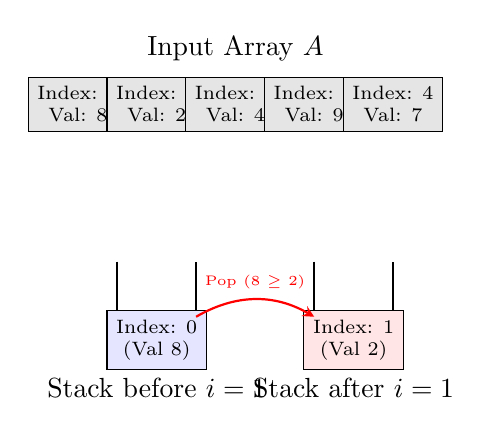
\begin{tikzpicture}[
  box/.style={draw, rectangle, minimum width=0.8cm, minimum height=0.6cm, font=\scriptsize, align=center},
  arrow/.style={->, >=stealth, thick}
]
% Draw input array
\node[box, fill=gray!20] (a0) at (0, 1.5) {Index: 0\\Val: 8};
\node[box, fill=gray!20] (a1) at (1, 1.5) {Index: 1\\Val: 2};
\node[box, fill=gray!20] (a2) at (2, 1.5) {Index: 2\\Val: 4};
\node[box, fill=gray!20] (a3) at (3, 1.5) {Index: 3\\Val: 9};
\node[box, fill=gray!20] (a4) at (4, 1.5) {Index: 4\\Val: 7};
\node at (2, 2.2) {Input Array $A$};

% Draw stack state before and after processing Index 1
\draw[thick] (0.5, -0.5) -- (0.5, -1.8) -- (1.5, -1.8) -- (1.5, -0.5);
\node[box, fill=blue!10] at (1, -1.5) {Index: 0\\(Val 8)};
\node at (1, -2.1) {Stack before $i=1$};

\draw[thick] (3.0, -0.5) -- (3.0, -1.8) -- (4.0, -1.8) -- (4.0, -0.5);
\node[box, fill=red!10] at (3.5, -1.5) {Index: 1\\(Val 2)};
\node at (3.5, -2.1) {Stack after $i=1$};

% Draw pop transition arrow
\draw[arrow, red, bend left] (1.5, -1.2) to node[above, font=\tiny]{Pop (8 $\ge$ 2)} (3.0, -1.2);

\end{tikzpicture}
\caption{Monotonic stack transition at $i=1$. The incoming element $A[1]=2$ is smaller than the top element $A[0]=8$, causing index 0 to be popped to maintain the increasing order property.}
\label{fig:monotonic_stack}
\end{figure}

\subsection{Java Implementation}
The optimal implementation is:
\begin{verbatim}
import java.util.Stack;

public class MonotonicStackSolver {
    public static int[] nearestSmallerElementLeft(int[] A) {
        Stack<Integer> st = new Stack<>(); // Stores indices
        int[] res = new int[A.length];
        
        for (int i = 0; i < A.length; i++) {
            // Maintain monotonic property
            while (!st.isEmpty() && A[st.peek()] >= A[i]) {
                st.pop();
            }
            // If empty, no smaller element on left
            res[i] = st.isEmpty() ? -1 : st.peek();
            // Push current index
            st.push(i);
        }
        return res;
    }
}
\end{verbatim}

\subsection{Complexity Analysis and Amortized Proof}
\begin{theorem}
The monotonic stack solver runs in $O(N)$ time.
\end{theorem}
\begin{proof}
Consider the operations on the stack. For each index $i \in [0, N-1]$, the index $i$ is pushed onto the stack exactly once. Each index $i$ can be popped from the stack at most once. Therefore, the inner \texttt{while} loop condition (which performs the \texttt{pop} operation) can evaluate to true at most $N$ times across the entire execution of the algorithm. Since the remaining operations inside the loop run in $O(1)$ time, the total time complexity is bounded by $O(N + N) = O(N)$.
\end{proof}

The space complexity is $O(N)$ auxiliary to store indices on the stack.

\subsection{Homework Extensions}
We extend this framework to two related problems:
\begin{enumerate}
    \item \textbf{Nearest Greater Element on Left:} Pop while $A[\mathtt{st.peek()}] \le A[i]$.
    \item \textbf{Nearest Smaller Element on Right:} Traverse the array from right to left (index $N-1$ down to $0$) maintaining the same logic.
\end{enumerate}

\section{Memory Management and Execution Lifecycle}
Understanding how the operating system manages memory during program execution is crucial for robust systems design.

\subsection{Stack vs. Heap Memory}
\begin{itemize}
    \item \textbf{Stack Allocation:} The call stack stores stack frames (activation records). Each stack frame holds local variables, parameters, and return addresses. Allocation is extremely fast (pointer increment) and automatically reclaimed upon function return.
    \item \textbf{Heap Allocation:} Used for dynamic memory. Programmers allocate heap space using \texttt{malloc} (C) or \texttt{new} (Java). Memory remains allocated until freed explicitly or garbage collected.
\end{itemize}

\subsection{Stack Overflow and Call Frames}
Each recursive call creates a new stack frame. If recursion lacks a base case, or exceeds maximum depth, the stack space is exhausted, triggering a \texttt{StackOverflowError}. In C, stack variables are limited in size; allocating a massive array on the stack (e.g., \texttt{int arr[10000000]}) can cause immediate segmentation faults.

\subsection{Parameter Passing and the Swap Pointer Fallacy}
Because parameters are passed by value in C, passing a pointer copy onto the stack frame of a function and swapping the pointer value there has no impact on the caller's stack frame. To persist pointer changes, one must pass double pointers (pointer-to-pointer, \texttt{Node**}), allowing dereferenced modifications to reach the caller's stack frame directly.

\section{Conclusion}
This paper presented a formal study of the stack data structure, its ADT definition, and standard representations. We analyzed key applications, establishing that balanced parenthesis checking and postfix evaluation operate in linear time. Finally, we demonstrated the power of the Monotonic Stack paradigm, showing how pruning redundant elements converts a naive $O(N^2)$ backward search into an optimal $O(N)$ solver. These stack concepts form the backbone of language compilers, virtual machines, and low-level runtime engines.

\end{document}
